\chapter*{Introducción}

Debido al desarrollo exponencial de la informática en el último siglo, todas las ramas del conocimiento se han visto afectadas. La informática está permitiendo la automatización de muchas tareas que anteriormente se realizaban de forma manual por un operario. 

Con el paso de los años, esta capacidad de automatización va en aumento pudiéndose aplicar en situaciones anteriormente impensables. Los numerosos avances en hardware y la aplicación de arquitecturas GPU en el campo del Aprendizaje Automático, y concretamente del Deep Learning, han permitido crear modelos mucho más avanzados capaces de interiorizar datos más complejos. 

La química es una de las ciencias que se ha impregnado de este desarrollo tecnológico y de esta combinación ha surgido lo que se conoce como cheminformatics o chemoinformatics. En este capítulo definiremos esta rama científica y describiremos sus principales actuaciones. A continuación, explicaremos distintos conceptos y tecnologías existentes relacionados con el proyecto.

\section*{Motivación del proyecto}
Desde hace décadas, en el mundo de la química ha estado presente la necesidad de almacenar, gestionar y procesar la gran cantidad de información que se genera. Con el tiempo se fueron desarrollando técnicas de tratamiento de ésta, pero no fue hasta hace algunos años cuando se acuñó el nombre de cheminformatics o chemoinformatics. 

En la literatura existen diferentes definiciones para este término, discutidas en \cite{doi:10.1021/ci600234z}. \\
``Chem(o)informatics es un término genérico que encompasa el diseño, creación, gestión, recuperación, análisis, diseminación, visualización y el uso de información química'' es una de las definiciones recogidas. Otra más abierta es ``La aplicación de métodos informáticos para resolver problemas de química''. 

% TODO: para qué necesitan los científicos de Negev un clasificador de imágenes?
Desde la Universidad de Granada, mi tutora Rocío trabaja en este ámbito. Colabora con químicos de la Universidad de Negev y es consciente de los problemas que tienen para manejar la gran cantidad de datos que aparecen en publicaciones científicas. Un tipo de datos muy valioso son las imágenes, pero clasificarlas no es trivial: pueden ser sobre cualquier temática, algunas pueden referirse a esquemas explicando cómo funciona un modelo, otras pueden contener resultados de algún experimento, pueden ser representaciones de compuestos químicos, etc. Clasificarlas manualmente por un operario no es una opción viable.

Es por ello que en este Trabajo de Fin de Grado vamos a crear una utilidad que permita clasificar imágenes. En concreto, aquellas que son representaciones de moléculas organometálicas, del resto.

Aunque existen diferentes opiniones sobre el alcance de las cheminformatics, se puede considerar que este proyecto está dentro de sus fronteras, ya que vamos a crear una herramienta de clasificación de imágenes químicas, es decir, una herramienta que procesa y analiza este tipo de información.

\section*{Compuestos orgánicos y su representación}
Un compuesto orgánico es un compuesto químico que contiene átomos de carbono, formando enlaces carbono-carbono y carbono-hidrógeno \cite{comporganico}. En este TFG, vamos a trabajar concretamente con la clasificación de compuestos organometálicos, donde los átomos de carbono forman enlaces covalentes con átomos metálicos \cite{comporganometalico}.

En las publicaciones de química encontramos numerosas representaciones gráficas de estos compuestos, lo que se conocen como fórmulas estructurales. Éstas muestran la disposición en el espacio de los átomos que forman el compuesto. Un ejemplo es la siguiente figura:

\begin{figure}[H]
\centering
    \fbox{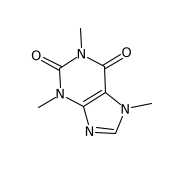
\includegraphics[scale=0.7]{imagenes/caffeine.png}}  
    \caption{Estructura de la cafeína} \label{fig:figura1}
\end{figure}

\noindent En ellas pueden aparecer multitud de elementos, apareciendo siempre:
\begin{itemize}
    \item \textbf{Átomos:} Se sitúan en los extremos de los enlaces. Representados con letras que indican el elemento químico del que se trata, tal y como aparece en la tabla periódica.
    \item \textbf{Enlaces:} Unen dos átomos entre sí. 
\end{itemize}

 En algunas ocasiones, sobre los átomos pueden mostrarse cargas positivas o negativas representando iones. Aparte, puede mostrarse lo que se conoce como información estereoquímica, que indica la disposición de los átomos en el espacio. Ésta es importante ya que afecta a las propiedades y reactividad de las moléculas \cite{estereoquimica,structrep}.

 \begin{figure}[H]
\centering
    \fbox{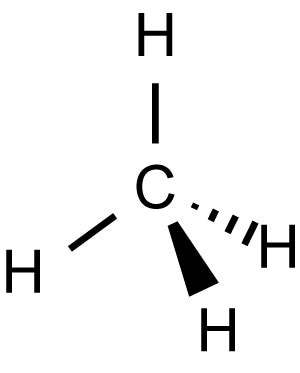
\includegraphics[scale=0.5]{imagenes/methane.jpg}}  
    \caption{Estructura del metano} \label{fig:figura2}
\end{figure}

\begin{itemize}
    \item Las líneas sólidas representan enlaces en el plano.
    \item Las discontinuas representan enlaces que están más alejados.
    \item Aquellas con forma de cuña indican que uno de los átomos se encuentra más cerca del espectador. 
\end{itemize}

Además, un mismo compuesto se puede representar de distintas formas:
\begin{figure}[H]
\centering
    \fbox{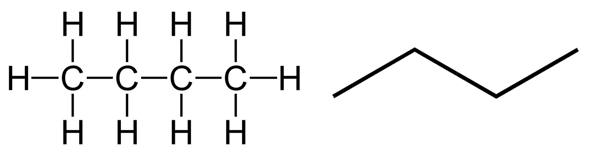
\includegraphics[scale=0.5]{imagenes/skeletal.png}}  
    \caption{Dos formas de representar el butano} \label{fig:figura2}
\end{figure}

A la izquierda se detalla la definición de todos los átomos, en cambio a la derecha encontramos lo que se conoce como fórmula de esqueleto, donde se omiten los átomos de carbono e hidrógeno. Se sabe que hay un átomo de carbono en los vértices que quedan libres en la intersección de dos enlaces o en las terminaciones donde no aparece ningún otro elemento. Se supone a la vez que cada átomo de carbono tiene cuatro enlaces, por tanto el número de enlaces que faltan por indicar explícitamente se corresponden con enlaces a moléculas de hidrógeno \cite{formestructural,structrep}.

